\subsection{Diagrammi di sequenza}
\begin{figure}[hb]
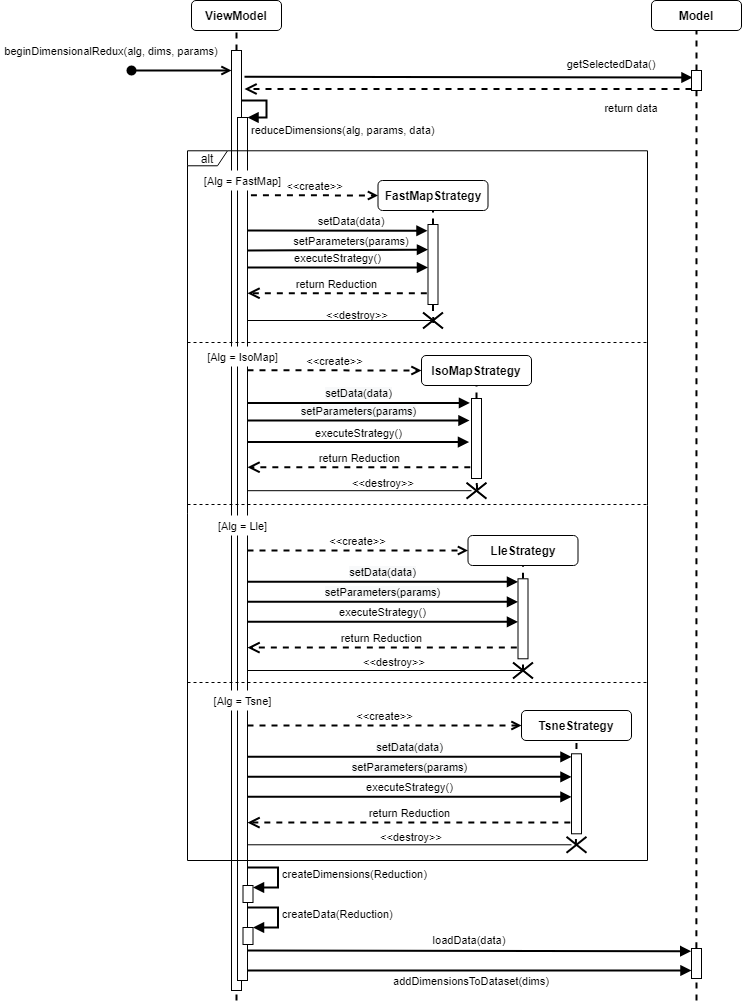
\includegraphics[width=12cm]{Images/Allegato Tecnico-Sequenza-DR}
\centering
\caption{Diagramma di sequenza che modella il processo di riduzione dimensionale}
\end{figure}
La funzione beginDimensionalRedux() è la funzione chiave per la riduzione dimensionale dei dati, essa viene chiamata nel ViewModel mentre l'utente interagisce con l'UI. Da qui il ViewModel ottiene i dati dal Model memorizzandoli nell'oggetto "data" per poi utilizzarli nella relativa Strategy (a seconda dell'algoritmo di riduzione scelto), alla quale vengono passati, oltre ai dati, i paramatri settati dall'utente.
Vengono quindi ritornati i dati ridotti, e usati per creare i nuovi array tramite i metodi createDimensions() e createData(), che verranno successivamente aggiunti al dataset iniziale.
\newpage
\begin{figure}[hb]
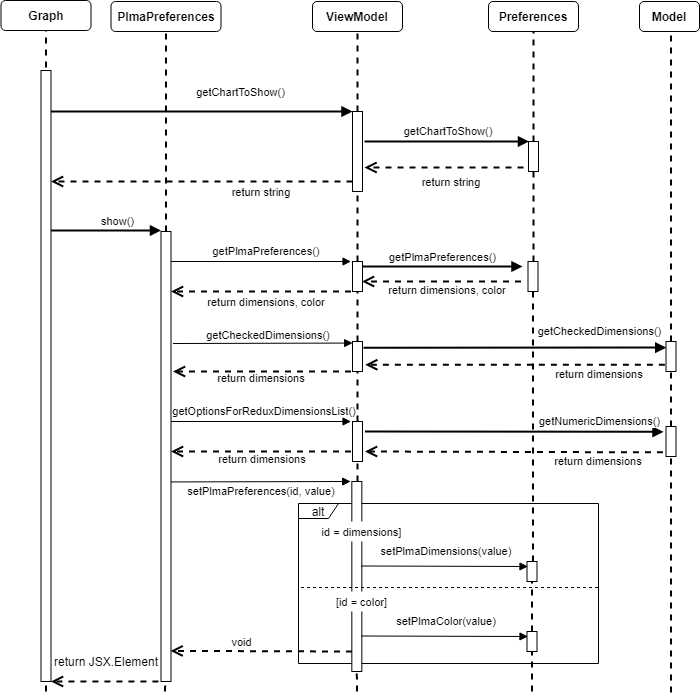
\includegraphics[width=14cm]{Images/Allegato Tecnico-Sequenza-PLMApref}
\centering
\caption{Diagramma di sequenza che modella il processo di visualizzazione delle preferenze per il grafico PLMA}
\end{figure}
Per semplicità è stato preso come esempio un singolo tipo di grafico, visto che per gli altri grafici vale lo stesso schema di funzionamento.
La funzione getChartToShow() viene chiamata ogni volta che nel modello avvengono delle modifiche, questa funzione mi ritorna una stringa con il nome del tipo di grafico da visualizzare, in questo caso quindi la stringa conterrà "PLMA".
Successivamente viene chiamata la funzione show() per mostrare a video un box con le preferenze scelte; questo chiama varie funzioni sulla ViewModel:
\begin{itemize}
\item getPlmaPreferences(), la quale ritorna le preferenze salvate in Preferences;
\item getCheckedDimensions(), la quale ritorna le dimensioni scelte, salvate in Model;
\item getOptionForReduxDimensionsList(), la quale ritorna le dimensioni scelte e non categoriche (necessarie per il PCA), salvate in Model;
\item setPlmaPreferences(), la quale salva le preferenze settate dall'utente in Preferences.
\end{itemize}
\newpage
\begin{figure}[hb]
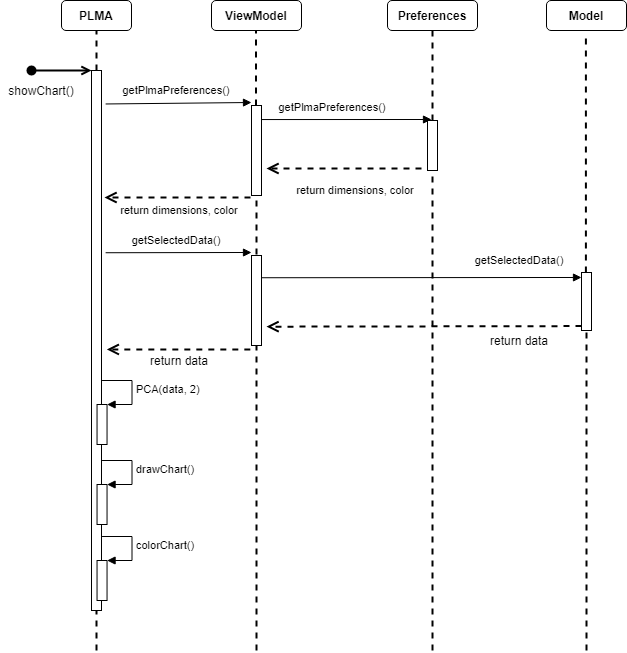
\includegraphics[width=15cm]{Images/Allegato Tecnico-Sequenza-PLMA}
\centering
\caption{Diagramma di sequenza che modella il processo per la visualizzazione del grafico PLMA}
\end{figure}
Per semplicità è stato preso come esempio un singolo tipo di grafico, visto che per gli altri grafici vale lo stesso schema di funzionamento.
showChart() è la funzione principale per richiamare la costruzione di un grafico, inizialmente vengono lette le preferenze settate dall'utente grazie al metodo getPlmaPreferences(), e vengono letti i dati da visualizzare grazie al metodo getSelectedData(). Successivamente viene invocato il PCA per avere le coordinate di partenza dei punti nel grafico (necessario per la visualizzazione del grafico PLMA). Infine il grafico viene disegnato tramite il metodo drawChart() e i punti vengono colorati tramite il metodo colorChart().

\newpage